\documentclass[twoside,11pt]{article}

%%%%% PACKAGES %%%%%%
\usepackage{pgm2016}
\usepackage{amsmath}
\usepackage{algorithm}
\usepackage[noend]{algpseudocode}
\usepackage{subcaption}
%\usepackage[utf8]{inputenc}		%NOT USED?
\usepackage[english]{babel}		%NOT USED?
\usepackage{paralist}			%NOT USED?
\usepackage[lowtilde]{url}
\usepackage{fixltx2e}
\usepackage{listings}
\usepackage{color}
\usepackage{hyperref}

\usepackage{auto-pst-pdf}
\usepackage{pst-all}
\usepackage{pstricks-add}



%%%%% MACROS %%%%%%
\algrenewcommand\Return{\State \algorithmicreturn{} }
\algnewcommand{\LineComment}[1]{\State \(\triangleright\) #1}
\renewcommand{\thesubfigure}{\roman{subfigure}}
\definecolor{codegreen}{rgb}{0,0.6,0}
\definecolor{codegray}{rgb}{0.5,0.5,0.5}
\definecolor{codepurple}{rgb}{0.58,0,0.82}
\definecolor{backcolour}{rgb}{0.95,0.95,0.92}
\lstdefinestyle{mystyle}{
   backgroundcolor=\color{backcolour},  
   commentstyle=\color{codegreen},
   keywordstyle=\color{magenta},
   numberstyle=\tiny\color{codegray},
   stringstyle=\color{codepurple},
   basicstyle=\footnotesize,
   breakatwhitespace=false,        
   breaklines=true,                
   captionpos=b,                    
   keepspaces=true,                
   numbers=left,                    
   numbersep=5pt,                  
   showspaces=false,                
   showstringspaces=false,
   showtabs=false,                  
   tabsize=2
}
\lstset{style=mystyle}

%%%%% SHORT HEADING %%%%%%
% Short headings should be running head and authors last names
\ShortHeadings{Beyond Quantum Computing: Are we living in a simulation}{dos Santos}
\firstpageno{1}

\begin{document}

\title{Research Task A - The Paper: \\ A Differential Approach to Inference in Bayesian Networks}

\author{\name Andr\'e E. dos Santos \email dossantos@cs.uregina.ca \\
\addr Department of Computer Science \\
University of Regina \\ 
Regina, Canada
}



\maketitle

\begin{abstract}%   <- trailing '%' for backward compatibility of .sty file
Bayesian networks (BNs) is a probabilistic graphical model for dealing with uncertainty in artificial intelligence.
However, BNs are known for requiring a high amount of processing during its running time of execution.
This strongly limits the applications of BNs to embedded systems, which are characterized for their primitive computational resources. 
\cite{darwiche00} proposes a new approach for inference in Bayesian networks based on partial differentiation.
Once the BN is processed, one can compute in constant-time answers to a large class of probabilistic queries.
One of the key contributions is the possible cost-effective implementation on a variety of software and hardware platforms.

The paper has a mathematical heavy notation and it is not a easy reading.
A reason is the weak background on probabilistic graphical models.
Thus, it is not self contained, which means one might have to look for second sources.
Throughout the paper, several advantages are presented
All claims have proof and are sound.
However, some points are not discussed in the paper, such the generalization of the proposed approach for other networks.
\end{abstract}


\section{Introduction}
\label{sec:intro}


We present a critique for the paper ``A Differential Approach to Inference in Bayesian Networks'', by \cite{darwiche00}.
The paper is the first of many published articles to present the idea of compiled BNs.
%\citep{darwiche2003differential,chavira2006compiling,park2004differential,chavira2007compiling}. 
It is also has been sum up as an important part of his book ``Modeling and Reasoning with Bayesian Networks'' \citeyearpar{darwiche2009modeling}.
The paper was published on the Proceedings of the Conference on Uncertainty in Artificial Intelligence (UAI).
UAI is yet today the leading conference of the field and is annually hold in the USA.
Some of its notorious sponsors are Google, Microsoft Research and Facebook.


Bayesian networks (BNs) \citep{pear88} is a probabilistic graphical model for dealing with uncertainty in artificial intelligence.
BNs overcame the acquisition intractability problem when reasoning with the a join probability distribution.
However, BNs are known for requiring a high amount of processing during its running time of execution \citep{koll09}.
This strongly limits the applications of BNs to embedded systems, which are characterized for their primitive computational resources. 
Due those limitations, consumer electronics often utilizes semantic weaker frameworks, such as Fuzzy logic or ruled-based systems.


\cite{darwiche00} proposes a new approach for inference in Bayesian networks based on partial differentiation.
Its first step is compiling the BN into a polynomial.
Then, it computes the partial derivatives of this polynomial with respect to each variable on the BN.
Once such derivatives are made available, one can compute in constant-time answers to a large class of probabilistic queries.
The differential approach presents two key contributions.
First, it enphasizes the role of partial differentiation on probabilistic reasoning, giving a new utility to central tasks of BNs.
Second, it helps the migration of BN applications to embedded systems, which are known for constraint in computational resources.

This paper is organized as follows.
%todo remainder
In Section \ref{sec:background}, Bayesian networks is reviewed.
Section \ref{sec:ac} presents ideas proposed in the paper.
The critique is drawn in Section \ref{sec:crt}.
Conclusions are given in Section \ref{sec:conc}.


\section{Background}
\label{sec:background}

A \emph{joint probability distribution} (JPD) is function $P$ on the Cartesian product $V$ of the variable domains such that the following two conditions hold: 
\begin{align}
	&0 \leq P(v) \leq 1.0\text{ for each configuration $v \in V$; and}\\		
	&\sum_{v \in V}{P(v)} = 1.0
\end{align}

Unlike \emph{fuzzy logic} and \emph{rule-based systems}, probability theory provides a rigorous mathematical foundation for the representation of uncertainty and for reasoning with uncertainty.
However, acquisition intractability is one of the problems of using only the jpd to model the problem domain.
For instance, specifying one probability value would be difficult with 50 variables, let alone 2\textsuperscript{50} probability values.

By exploiting the notion of \emph{probabilistic conditional independence}, \cite{pear88} solved the jpd acquisition problem by introducing Bayesian networks.
A \emph{Bayesian network} (BN) \cite{pear88} is a directed acyclic graph (DAG) on finite set of discrete variables $U$ together with \emph{conditional probability tables} (CPTs) $P(v_1 | Pa(v_1))$, $P(v_2|Pa(v_2))$, $\ldots$, $P(v_n|Pa(v_n))$,
where $Pa(v_i)$ denotes the parents of the variable $v_i$ in the DAG.
The product of the CPTs for the DAG on $U$ is a \emph{joint probability distribution} $P(U)$ \citep{pear88}.
For example, Figure \ref{fig:bn} shows a Bayesian network with CPTs $P(a)$ and $P(b|a)$ in Table 1.


\begin{figure}[htbp]
\centering
 \psset{unit=1cm}
      \begin{pspicture}(0,0.5)(2,3)%\showgrid
        \rput(2,1){\ovalnode{X1}{$B$}}
        \rput(0,1){\ovalnode{X2}{$A$}}
        
        \ncline{->}{X2}{X1}
         
  \end{pspicture}
%\includegraphics[page=1]{amidst_T41-pics.pdf}
\caption{A BN from \citep{darwiche00}.}
\label{fig:bn}
\end{figure}

\begin{table}[!htb]
    \label{subtb:pa}
    \caption{Table (a) provides the prior probability of variable $A$ and Table (b) provides the conditional probability of $B$ given $A$.}
    \begin{subtable}{.5\linewidth}
      \centering
        \caption{}
        \begin{tabular}{c|c}
            $A$ & $P(A)$ \\ \hline
            1 & 0.3 \\
            0 & 0.7
        \end{tabular}
    \end{subtable}%
    \begin{subtable}{.5\linewidth}
      \centering
        \caption{}
        \begin{tabular}{cc|c}
            $A$ & $B$ & $P(B|A)$ \\ \hline
            1 & 1 & 0.1 \\
            1 & 0 & 0.9 \\
            0 & 1 & 0.8 \\
            0 & 0 & 0.2 \\
        \end{tabular}
    \end{subtable} 
\end{table}


Unfortunately, both exact and approximate inference in Bayesian networks are, in general,  \emph{NP-hard} \citep{koll09}. 
Thus, the use of exponential complexity algorithms is justified.
That implies a limitation for BN applications to embedded systems, which are known for constraint in computational resources.

\section{A Differential Approach to Inference in Bayesian Networks}
\label{sec:ac}


In this section we show the mains ideas proposed by the paper ``A Differential Approach to Inference in Bayesian Networks'' \citeyearpar{darwiche00}.
We give an overview on how to  represent a BN as a polynomial, and then compiling and evaluating the polynomial representation.

\subsection{Polynomial Representation of Bayesian networks}

We now show how to represent a BN as a polynomial $\cal F$ that includes two type os variables:
evidence indicator $\lambda$ and
network parameter $\theta$ (probability values).

We can parameterize a CPT as follows.
A \emph{parameterize} table receives a evidence indicator $\lambda$ multiplied to the probability value.
For instance, Table 2 shows the parameterized CPTs for the BN of Table 1.
Notice that $\bar x$ denotes the instantiation $x = 0$.

\begin{table}[!htb]
    \caption{Table (a) provides the parameterized CPT for $P(A)$ and Table (b) provides the parameterized CPT for $P(B|A)$.}
    \begin{subtable}{.5\linewidth}
    \label{subtb:papara}
      \centering
        \caption{}
        \begin{tabular}{c|c}
            $A$ & $P(A)$ \\ \hline
            1 & 0.3$\lambda_{{A}}$ \\
            0 & 0.7$\lambda_{\bar{A}}$
        \end{tabular}
    \end{subtable}%
    \begin{subtable}{.5\linewidth}
      \centering
        \caption{}
        \begin{tabular}{cc|c}
            $A$ & $B$ & $P(B|A)$ \\ \hline
            1 & 1 & 0.1$\lambda_{{B}}$ \\
            1 & 0 & 0.9$\lambda_{\bar{B}}$ \\
            0 & 1 & 0.8$\lambda_{{B}}$ \\
            0 & 0 & 0.2$\lambda_{\bar{B}}$ \\
        \end{tabular}
    \end{subtable} 
\end{table}

The polynomial $\cal F$ of a BN is represented by the formula:
\begin{align}
	{\cal F}(\lambda,\theta) = \sum_{U}{\prod{\theta_i}\prod{\lambda_i}}
\end{align}

As an example, the polynomial of the BN in Figure 1 is

\begin{align}
	{\cal F} = \theta_{A}\theta_{B|A}\lambda_{A}\lambda_{B} +
	  \theta_{A}\theta_{\bar{B}|A}\lambda_{A}\lambda_{\bar{B}} +
	 \theta_{\bar{A}}\theta_{B|\bar{A}}\lambda_{\bar{A}}\lambda_{B} +
	  \theta_{\bar{A}}\theta_{\bar{B}|\bar{A}}\lambda_{\bar{A}}\lambda_{\bar{B}}
\end{align}

The size of the polynomial is exponential to the size of the network.

Now, with a evidence we can set a indicator $\lambda$ to either 0 or 1.
If is consistent with the evidence is 1, and is 0 otherwise.
For example, if the evidence is $A\bar{B}$ that is, $A$ is true, $B$ is false, then
	${\cal F}(
	\lambda_{A}=1,
	\lambda_{\bar{A}}=0,
	\lambda_{B}=0,
	\lambda_{\bar{B}}=1,
	\theta_{A} = 0.3,
	\theta_{\bar{A}} = 0.7,
	\theta_{B|A} = 0.1,
	\theta_{\bar{B}|A} = 0.9,
	\theta_{B|\bar{A}} = 0.8,
	\theta_{\bar{B}|\bar{A}} = 0.2,			
	)$,
which equal to 0.27 in this case.
The probability values are the correspondents in the respectively CPTs.
Therefore, the polynomial is a linear function of many variables, where each one corresponds to either an evidence indicator $\lambda$ or a probability value $\theta$.
Each parameter has degree one.
For each instantiation given an evidence, the polynomial can be evaluated to compute the probability of the variable given the evidence.

The author highlights that BNs represented by polynomial function has been already exploited by other authors \citep{castillo1996goal,castillo1997sensitivity,russell1995local}.
However, the evidence indicators were fixed to a particular value.
Hence, they  could not be used to answer queries with respect to varying evidence.


\subsection{Compiling a Bayesian networks}

The paper presents a algorithm, called $\Call{VE\_COMPLETE}{}$, to compile a polynomial representation of a BN. 
$\Call{VE\_COMPLETE}{}$ receives as input a BN and an elimination ordering of the variables.
The result is a more compact polynomial following the elimination ordering used to construct this new presentation.
Thereby, a rooted DAG can be drawn for the compiled polynomial.
For instance, the compiled polynomial in (4) following the elimination ordering $\{B,A\}$ is
\begin{eqnarray}
	{\cal F} = \theta_{A}\lambda_{A}(\theta_{B|A}\lambda_{B} + \theta_{\bar{B}|A}\lambda_{\bar{B}}) + \theta_{\bar{A}}\lambda_{\bar{A}}(\theta_{B|\bar{A}}\lambda_{B}+\theta_{\bar{B}|\bar{A}}\lambda_{\bar{B}})
\end{eqnarray}
and depicted in Figure \ref{fig:comp}.

\begin{figure}[!htb]
    \begin{center}
    	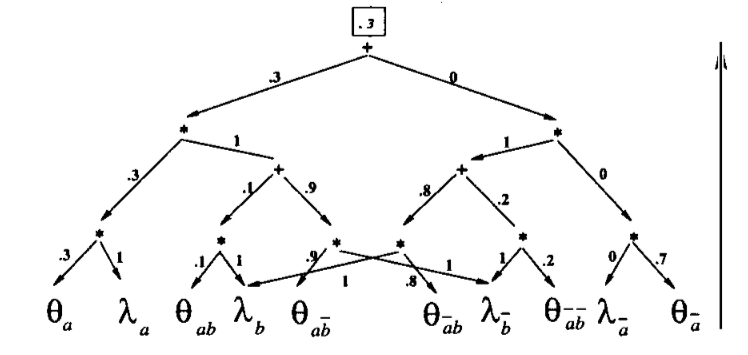
\includegraphics[width=\columnwidth]{figures/compiled.png}
		\caption{Rooted DAG representing Equation (5).}
		\label{fig:comp}
    \end{center}
\end{figure}


\subsection{Evaluating and Differentiating a Polynomial Representation}

The evaluation of the complied polynomial and computing the partial derivatives is a two-phase message passing scheme in which each message is simply a number.
The first phase, massages are sent from nodes to their parents in the rooted DAG following the operations of each node.
Figure \ref{fig:comp} shows this process, where it leads to assigning the value 0.3 to the root, indicating that the probability of evidence $E$ is $P(E) = 0.3$.
Second phase, messages are sent from nodes to children in the same rooted DAG, leading to computation of all partial derivatives.
This processes is illustrated in Figure \ref{fig:deri}.

\begin{figure}[!htb]
    \begin{center}
    	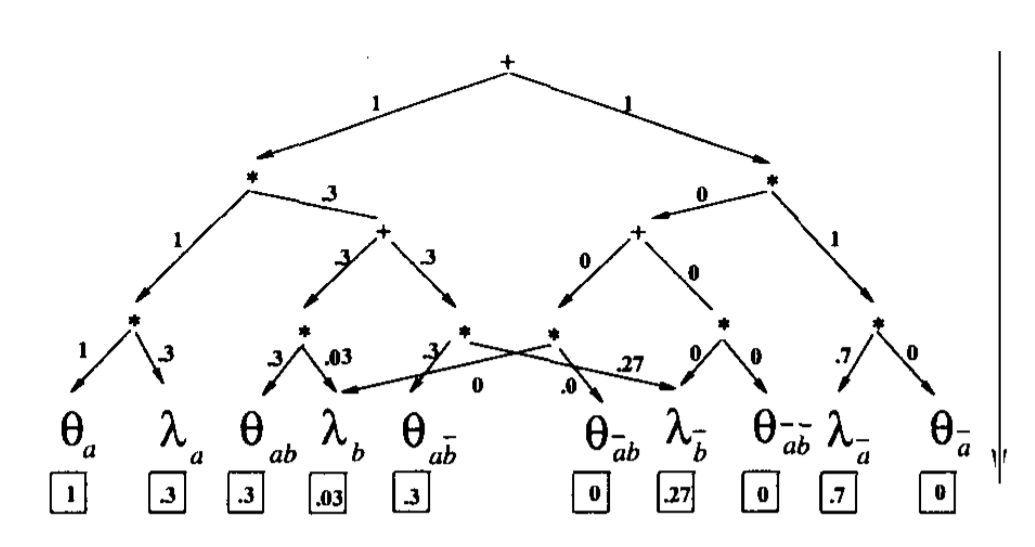
\includegraphics[width=\columnwidth]{figures/deriv.png}
		\caption{Second phase of the evaluation of rooted DAG in Figure 5, under evidence $E=A$.}
		\label{fig:deri}
    \end{center}
\end{figure}

The number of messages passed in both phases is twice the number of edges in the compilation of the polynomial.
Since each message can be computed in constant time, the whole computation is linear in the size of the polynomial.

After the two-phase steps we have the capacity to answer, in constant time, a very large class of probabilistic queries, relating to classical inference, parameter estimation, model validation and sensitivity analysis.
Some of those queries are
(i) in the root node the probability of the evidence, and 
(ii) the posterior marginal of any network variable.

\section{Criticism}
\label{sec:crt}

In this section we present a critique for the paper ``A Differential Approach to Inference in Bayesian Networks'' \citep{darwiche00}.

The paper is well written and presents a good flow of ideas.
Even so, the paper has a mathematical heavy notation and it is not a easy reading.
The background on probabilistic graphical models is not provided.
For instance, Section 2 of this paper was drawn from my personal knowledge of the field.
Thus, the paper is not self contained, which can lead some readers to search for second sources.


The paper presents several advantages.
Proofs are provided and state the soundness of the mathematical claims.
However, some points are not discussed
For instance, the generalization of the proposed approach for other networks and how to deal with intractable networks are not discussed. 
Even thought the author being known for several winnings with his application on the Probabilistic Inference Competition of the proceedings, the paper also does not present experimental results to endure its claims.
There is a typo on the Section 1, first result of the paper: ``Given a variable elimination order of \emph{with} $w$ [...]'', the correct word is \emph{width}.
On the polynomial representation example, the the third network parameter $\theta_{B|A}$ should be $\theta_{B|\bar{A}}$.


The main advantage of the paper is to simplify inference systems to the point where they could be implemented cost-effectively on a variety of software and hardware platforms.
That would allow emmbeded systems that normally uses Fuzzy logic or rule-based system to starts using BNs, a more powerful semantic tool for dealing with uncertanty.
And with the advantage not requiring a lot of processing during running time of execution
This is a direct drawn from the three main results of the paper:
(i) compiling the polynomial in linear in the size of the polynomial,
(ii) answering a large number of queries by (i), and
(iii) computing the partial derivatives of $\lambda$ and $\theta$ simultaneously in time linear in the size of the polynomial.

There is no doubt the paper presents a breakthrough on BNs field.
The author even states that the he is not aware of any computational framework for BNs, which combines the simplicity, comprehensiveness and computational complexity of the presents framework based on partial derivatives.
%However, after network polynomials \citep{darwiche00}, \cite{poon2011sum} generalized network polynomials to unnormalized distributions and has been the ``state of the art'' on probabilistic graphical models.

 
\section{Conclusion}
\label{sec:conc}

We have presented an overview and critique of the paper ``A Differential Approach to Inference in Bayesian Networks'' by \cite{darwiche00}.
The main advantage of the paper is to simplify inference systems to the point where they could be implemented cost-effectively on a variety of software and hardware platforms.
The differential approach presents two key contributions.
First, it enphasizes the role of partial differentiation on probabilistic reasoning, giving a new utility to central tasks of BNs.
Second, it helps the migration of BN applications to embedded systems, which are known for constraint in computational resources.

\cite{darwiche00} proposes a new approach for inference in Bayesian networks based on partial differentiation.
Its first step is compiling the BN into a polynomial.
Then, it computes the partial derivatives of this polynomial with respect to each variables.
The partial derivatives are important when estimating BN parameters and when performing sensitivity analysis.
Moreover, with the derivatives it is possible to compute in constant-time answers to a large class of probabilistic queries.

The paper presents a breakthrough on BNs field, which may lead let to new (more comprehensive) networks. 
%\citep{poon2011sum}.
However, the differential approach to inference in BNs was the first computational framework to combine partial derivatives for such a purpose.
That has been leading to a great advancements on the field and made more viable BN applications to embedded systems.

\vskip 0.2in
\bibliography{references/references}
\end{document}
